\section{Multi-microphone beamforming} \label{sec:mm_bf}
When using multiple microphones, the spatial properties of the incomming signals can be exploited. Since there is a (small) but relevant  distance difference between the microphones, the time of arrival of the same signal differs. This time delay can be used to estimate the direction of the source and to filter other (interfering) directions.

Before the system is designed and the signals are discussed, some assumptions are made. First of all, the speech and noise are assumed to be  WSS. Secondly a far field is assumed where the angles of arrival at every microphone is identical. These two assumptions can be used to simplify the incoming signals at each microphones. Since the signal is WSS, a time delay can be interpreted as a pahse shift in frequency.

Because there is a phase shift, spatial aliasing becomes important. This is where distance between microphones become too big where the periodic signal shifts a full time interval. To avoid this, the distance between microphones should be smaller than half of the wavelength. When assuming a maximum frequency of 8000KHz, the maximum distance between microphones is 2 milimiters.

Since the signal only differs in phase and a linear microphone setup, the signal model for each microphone can be defined as in Eq. \ref{eq:bf}.

\begin{equation}
  \mathbf{Y}_{k}(l) =
  \begin{bmatrix}
    S_{k}(l) & S_{k}(l)e^{-j2\pi\frac{k\tau}{N}} & \hdots & S_{k}(l)e^{-j2\pi(M-1)\frac{k\tau}{N}}
  \end{bmatrix}
  + \mathbf{N}_{k}(l)
  \label{eq:bf}
\end{equation}

In this equation, $\mathbf{Y}_{k}(l)$ can be expressed as a linear combination of $S_{k}(l)$ by a steering vector defined in Eq. \ref{eq:steering}. The resulting model can then be expressed as showed in Eq. \ref{eq:bf_model}.

\begin{equation}
  \mathbf{d}_{k} =
  \begin{bmatrix}
    1 & e^{-j2\pi \frac{k\tau}{N}} & \hdots & e^{-j2\pi(M-1)\frac{k\tau}{N}}
  \end{bmatrix}
  \label{eq:steering}
\end{equation}

\begin{equation}
  \mathbf{Y}_{k}(l) = S_{k}(l)\mathbf{d}_{k} + \mathbf{N}_{k}(l)
  \label{eq:bf_model}
\end{equation}

From this last model, the source signal can easily opbtained by the equation shown in Eq. \ref{eq:bf_sol}. This method is called the delay and sum beamformer, since the first signals are delayed untill all the signals can be added. Results and performance of this beamforer is showed in Fig. \ref{fig:bf}. Where nine microphones were used with a initial SNR of 5 dB and an angle of arival at 90 degrees.

\begin{equation}
   \hat S_{k}(l) =\frac{1}{M} \mathbf{d}_{k}^{H}\mathbf{Y}_{k}(l)
  \label{eq:bf_sol}
\end{equation}

\begin{figure}
  \centering
  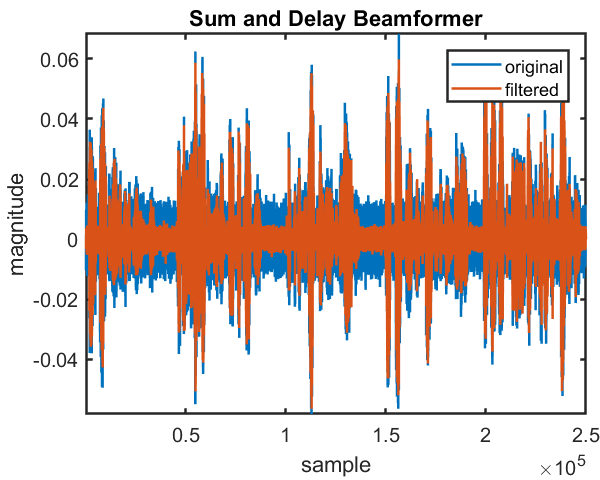
\includegraphics[width=0.5\textwidth]{images/beamformer_sum_delay.png}
  \caption{Performance of the delay and sum beamformer.}
  \label{fig:bf}
\end{figure}
